\chapter{Solução e Avaliação da Proposta}
\section{Solução Proposta}
Esta seção é destinada a explicação de como você resolverá o problema, ou como você pretende
realizar o projeto. Neste estágio é preciso estar claro o que você irá fazer, mas flexível o
suficiente para adaptar a solução a adversidades encontradas durante a realização do projeto. A
escrita da proposta da solução não o previne do insucesso, mas permite que você identifique
diversos problemas com antecedência. Note que a metodologia descrita aqui é dependente do tipo
de projeto do seu TCC. Você deve discutir com seu orientador sobre isso.

Conforme a Figura \ref{fig:controlepfc3ph}, o controle do PFC trifásico

\begin{figure}
    \centering
    \caption{Esquema de controle do PFC trifásico.}
    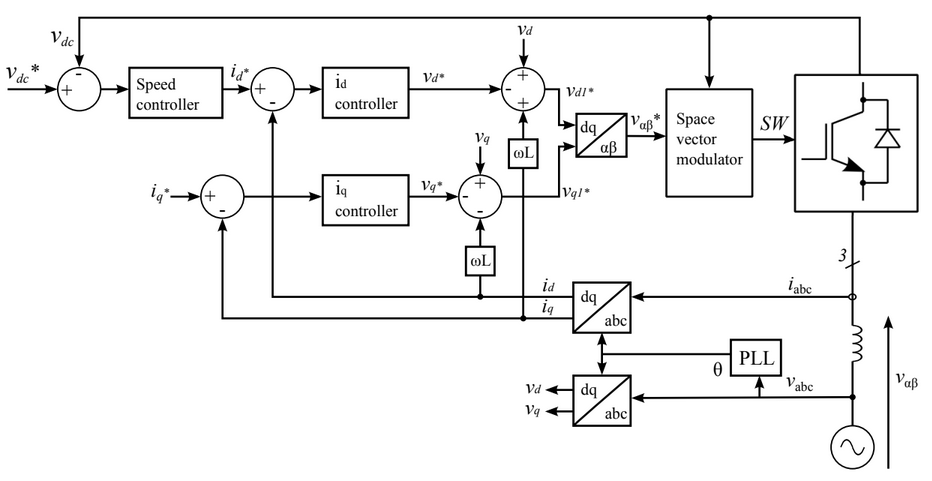
\includegraphics[width=0.8\textwidth]{./Figuras/controlepfc3ph.png}
    \legend{Fonte: \cite{3phPlecs}.}
    \label{fig:controlepfc3ph}
\end{figure}

\section{Avaliação da Solução}
Esta seção deve conter uma explicação de como será feita a avaliação da solução uma vez que ela
estiver concluída. O método de avaliação é dependente do projeto e o seu orientador pode
guiá-lo para a forma de avaliação mais adequada.
